\section{Simple Grid Method}
\label{sec:simple_grid_method}

The simplest method for analysing the distribution of points is to use a
regular grid of cells and place the points into the cells one at a time. Once
all points have been added, the number of points per cell can be treated as a
greyscale birghtness value. A thresholding filter can then be applied to remove
the points that are isolated. The implementation to acheive this outputs a
single pixel value for each of the cells of the grid. If written to a file,
this can easily be viewed by treating the resulting file as an pnm image
format.

Though the resolution of this method can be easily changed by altering the size
of the cells, it performs badly when presented with data that is even slightly
noisy. If the clusters themselves have a density that is not significantly
above the background noise level, the thresholding step is prone to either
exclude much of the real data, or to increase the size of the clusters by
including too much noise. These two effects can be seen clearly in
figure~\ref{fig:grid-noise}, where \texttt{palm-1.txt} was used with a cell
size of 200.

\begin{figure}[ht]
    \centering
    \begin{subfigure}[b]{0.4\textwidth}
        \frame{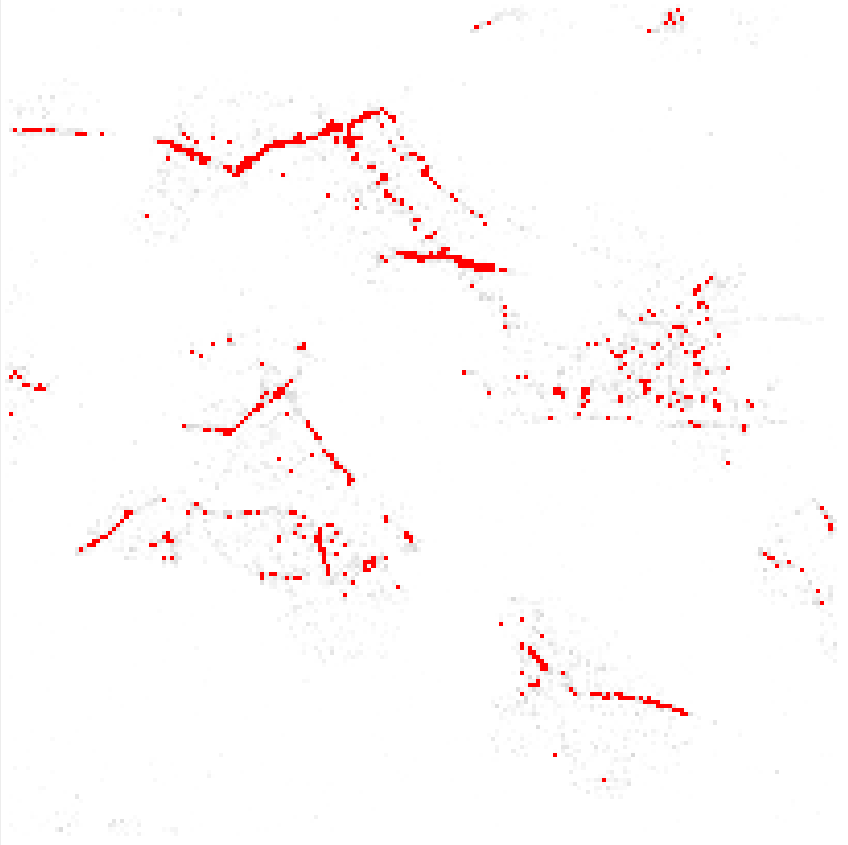
\includegraphics[width=\textwidth]{grid-noise-low.png}}
        \caption{}\label{fig:grid-noise-low.png}
    \end{subfigure}%
    \qquad
    \begin{subfigure}[b]{0.4\textwidth}
        \frame{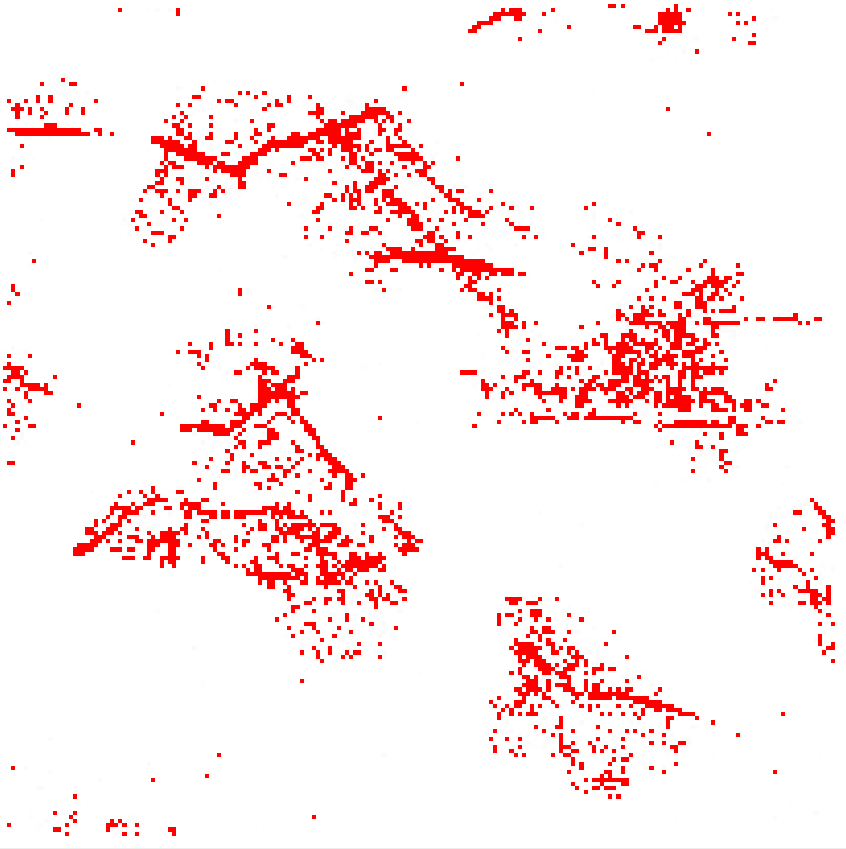
\includegraphics[width=\textwidth]{grid-noise-high.png}}
        \caption{}\label{fig:grid-noise-high.png}
    \end{subfigure}
    \caption{Setting a low threshold, \subref{fig:grid-noise-low.png}, means
    that many of the points in the clusters are lost. Setting it higher,
    \subref{fig:grid-noise-high.png}, includes too many of the points deemed to
    be noise.}\label{fig:grid-noise}
\end{figure}
